null
\chapter[REFERENCIAL TE\'ORICO]{ REFERENCIAL TE\'ORICO}

\bigskip

{
Durante o desenvolvimento do nosso projeto, utilizamos de algumas ferramentas de apoio ao desenvolvimento adequado ao
nosso tipo software, entre elas {\LaTeX},\ NetBeans IDE, APIs Java como Writer2Latex e \ JLR (Java Latex Report),
Tamb\'em utilizamos a metodologia Extreme Programming (XP). Neste cap\'itulo falaremos sobre cada uma dessas
ferramentas e metodologias.}


\bigskip

\section[XP {}-- EXTREME PROGRAMMING]{ XP -- EXTREME PROGRAMMING}

\bigskip

{
O Extreme Programming (XP)\ foi criado em 1997 por Kent Beck. ``A Extreme Programming (XP) \'e uma metodologia \'agil
para equipes pequenas e m\'edias que desenvolvem software baseado em requisitos vagos e que se modificam rapidamente''
(BECK, 2000).}

{
O XP visa garantir a satisfa\c{c}\~ao do cliente, enfatizando o desenvolvimento \'agil do projeto para o cumprimento das
estimativas e vem ocupando espa\c{c}o consider\'avel no mercado, que antes que antes era dominado por metodologias
tradicionais, como RUP -- Rational Unified Process.}

{
Este subcap\'itulo tem como objetivo fazer uma breve apresenta\c{c}\~ao dessa metodologia, seus valores e algumas de
suas pr\'aticas para justificar a utiliza\c{c}\~ao da mesma nesse projeto, evitando uma abordagem detalhada e
desnecess\'aria ao objetivo do projeto.}


\bigskip

{
VALORES XP}


\bigskip

{
{}``Metas\ individuais de curto prazo frequentemente entram em conflito com metas s\'ocias de longo prazo. As sociedades
aprenderam a lidar com esse problema desenvolvendo um conjunto de valores a serem compartilhados'' (BECK, 2000).
Extreme Programming possui cinco valores a partir dos quais s\~ao desenvolvidas todas as suas pr\'aticas.}


\bigskip

{
Esses s\~ao os cinco valores de XP:}

\liststyleLFOi
\begin{itemize}
\item {
\textrm{\textbf{Comunica\c{c}\~ao:}}\textrm{\ deve ser priorizado o di\'alogo presencial que melhora o entendimento
tanto entre cliente e desenvolvedor quanto dentro da pr\'opria equipe de desenvolvimento;}}
\item {
\textrm{\textbf{Simplicidade:}}\textrm{\ desenvolver apenas o que \'e essencial ao software evita que se produza algo
que n\~ao utilizado. Vale mais a pena adicionar modifica\c{c}\~oes a desenvolver c\'odigos in\'uteis;}}
\item {
\textrm{\textbf{Feedback:}}\textrm{\ quanto mais cedo for identificada a necessidade de mudan\c{c}as mais barato ser\'a
para o desenvolvedor e para o cliente aplica-las. Feedback constante permite a r\'apida identifica\c{c}\~ao de
poss\'iveis erros e da necessidade de mudan\c{c}as ou melhorias no software;}}
\item {
\textrm{\textbf{Respeito:}}\textrm{\ todos devem ser respeitados igualmente dentro e\ fora da equipe, pois todos
contribuem com o desenvolvimento. Todo o tipo de experi\^encia e conhecimento deve ser respeitado;}}
\item {
\textrm{\textbf{Coragem:}}\textrm{\ \'e necess\'aria para estar preparado para as constantes mudan\c{c}as que podem
ocorrer em um projeto de software, bem como para aplicar todos os valores de XP.}}
\end{itemize}

\bigskip

{
Pr\'aticas XP}


\bigskip

{
Cada uma das pr\'aticas de Extreme Programming visa atender um ou mais dos valores citados acima e n\~ao possuem nenhum
valor se n\~ao forem usadas buscando atender esses valores. Cada pr\'atica aplicada separadamente gera benef\'icios ao
projeto, mas a utiliza\c{c}\~ao de v\'arias pr\'aticas em conjunto pode-se notar um ganho de benef\'icios muito maior.}


\bigskip

{
Listaremos a seguir algumas pr\'aticas de XP que foram adotadas por essa equipe com uma breve descri\c{c}\~ao das
mesmas:}

\liststyleLFOii
\begin{itemize}
\item {
\textrm{\textbf{Cliente Presente:}}\textrm{\ o cliente faz parte da equipe do desenvolvimento de software e \'e
presen\c{c}a constante nesse processo, fornecendo feedback com a maior frequ\^encia poss\'ivel;}}
\item {
\textrm{\textbf{Jogo do Planejamento:}}\textrm{\ planejamento \'e uma atividade cont\'inua desempenhada durante todo o
projeto, esta\ postura admite que ao longo do projeto as prioridades e necessidades do cliente sofrem constantes
mudan\c{c}as, portanto o planejamento deve acompanhar essas mudan\c{c}as;}}
\item {
\textrm{\textbf{C\'odigo Coletivo:}}\textrm{\ todo o desenvolvedor tem\ acesso a todas as partes do c\'odigo
(inclusive\ aquelas que ele n\~ao programou) e podem fazer qualquer altera\c{c}\~ao sem ter que pedir permiss\~ao,
desde que haja necessidade de tal altera\c{c}\~ao;}}
\item {
\textrm{\textbf{Integra\c{c}\~ao Cont\'inua:\ }}\textrm{\'e feita constantemente a integra\c{c}\~ao do c\'odigo
produzido ao restante do sistema\ assegurando, ao final de cada integra\c{c}\~ao, a consist\^encia da base de
c\'odigo.}}
\item {
\textrm{\textbf{Ritmo Sustent\'avel:}}\textrm{\ recomenda que os membros da equipe trabalhem oito horas por dia e evitem
ao m\'aximo a utiliza\c{c}\~ao de horas-extras de trabalho.}}
\item {
\textrm{\textbf{Projeto Simples:}}\textrm{\ {}``o sistema deve ser projetado da maneira mais simples o poss\'ivel em
qualquer momento. A complexidade desnecess\'aria \'e removida assim que for descoberta'' (BECK,2000).}}
\end{itemize}
{
O usu\'ario de XP n\~ao tem a obriga\c{c}\~ao de aplicar todas as suas pr\'aticas, mas apenas aquelas que se adequarem
as necessidades do projeto.}


\bigskip

\subsection[Por que utilizamos XP]{ Por que utilizamos XP}

\bigskip

{
Decidimos aplicar XP devido a sua flexibilidade para com poss\'iveis mudan\c{c}as no decorrer do projeto e a
possibilidade de escolher e adaptar as pr\'aticas de XP as necessidades de nosso projeto e as restri\c{c}\~oes de nossa
equipe.}

{
Possu\'iamos tamb\'em um grande interesse, pessoal e profissional, em conhecer, aprender e aplicar essa metodologia que
vem ganhando espa\c{c}o no mercado de desenvolvimento de software.}


\bigskip

\section[LaTeX]{ {\LaTeX}}

\bigskip

{
{}``LATEX \'e um sistema para formata\c{c}\~ao de textos de documentos. Sua primeira vers\~ao amplamente dispon\'ivel,
misteriosamente numerada 2.09, apareceu em 1985{\textquotedbl} (LAMPORT, 1995)}

{
O {\LaTeX} \'e um pacote de macros para desenvolver e gerar documentos para impress\~ao com alta qualidade
tipogr\'afica, criado por Leslie Lamport e mantido por Frank\ Mittelbach atualmente, podendo ser utilizado um layout
profissional predefinido. O seu desenvolvimento usou o TeX como motor de formata\c{c}\~ao.}

{
TeX \'e um software da onde se originou o LaTex, foi desenvolvido por Donald E. Knuth que come\c{c}ou a escrev\^e-lo em
1977, \'epoca em que editoras gr\'aficas come\c{c}aram a utilizar equipamentos digitais para impress\~ao.}

{
Segundo Knuth (1984) ao ``preparar um manuscrito em formato TEX, voc\^e estar\'a dizendo a um computador exatamente como
o manuscrito deve ser transformado em p\'aginas cuja qualidade aparenta ser tipogr\'afica''.}

{
\textrm{Os caracteres T, E, X no nome derivam respectivamente das letras gregas tau, \'epsilon, e chi, como o nome do
TeX deriva do grego\ }\textrm{\textit{$\tau \text{\textgreek{'e}}\chi \nu \eta $}}\textrm{\ (habilidade, arte,
t\'ecnica) a sua pron\'uncia correta\ }\textrm{seria ``t\'ec''. J\'a a primeira s\'ilaba do nome se pronuncia
exatamente igual \`a palavra inglesa lay sendo a pronuncia correta para {\LaTeX} \'e ``lei-t\'ec''.}}


\bigskip

\subsection[Benef\'icios do Latex]{ Benef\'icios do Latex}

\bigskip

{
\textrm{Para o usu\'ario comum, que n\~ao conhece ou apenas ouviu falar do Latex, imediatamente deve se perguntar,
``esse \'e mais um\ processador de texto, mas porque devo usar?''. Alguns pontos para essa pergunta.}}


\bigskip

\liststyleLFOiii
\begin{itemize}
\item {
\textrm{Devido aos seus layouts padronizados, os textos nele baseado possuem uma apar\^encia de texto de gr\'afica;}}
\item {
O Latex e totalmente gratuito e pode funcionar em quase todas as\ plataformas;}
\item {
Produ\c{c}\~ao de textos estruturados;}
\item {
N\~ao \'e necess\'ario montar um layout para uso personalizado, o usu\'ario precisa apenas conhecer alguns comandos que
estruturam o documento;}
\item {
A constru\c{c}\~ao de f\'ormulas matem\'aticas, tabelas, refer\^encias, rodap\'es, \'indices no {\LaTeX} \'e totalmente
facilitado;}
\item {
O padr\~ao Latex \'e amplamente usado pela comunidade acad\^emica e cient\'ifica, sendo em alguns casos obrigat\'orio o
seu uso em trabalhos acad\^emicos.}
\end{itemize}

\bigskip

\subsection[Por que utilizamos LaTeX]{ Por que utilizamos {\LaTeX}}

\bigskip

{
Devido aos benef\'icios j\'a citados, o {\LaTeX} \'e muito\ utilizado em Universidades e Empresas de m\'edio e grande
porte para o desenvolvimento de relat\'orios, monografias, artigos e demais documentos que requerem um alto n\'ivel de
padroniza\c{c}\~ao.}

{
Observamos que o desenvolvimento do TCC demanda muito tempo dos alunos\ e a necessidade de aprender uma tecnologia
desconhecida para a maioria dos alunos apenas para desenvolver a documenta\c{c}\~ao do TCC limitava o tempo de trabalho
dos mesmos.}

{
Neste trabalho temos como objetivo principal desenvolver um software que intermediasse\ a intera\c{c}\~ao entre um aluno
que esteja desenvolvendo um TCC e o {\LaTeX}, tornando o processo de desenvolvimento do TCC mais intuitivo e isentando
o aluno da necessidade de aprender {\LaTeX} para desenvolver um TCC, com nosso programa sendo o instrumento para a\ sua
documenta\c{c}\~ao final.}


\bigskip

\section[AS CLASSES ABNTeX E ABNTeX2]{ AS CLASSES ABNTeX E ABNTeX2}

\bigskip

{
\textrm{O {\LaTeX}, usado amplamente pela comunidade acad\^emica para produ\c{c}\~ao de textos matem\'aticos e
cient\'ificos, n\~ao possu\'ia uma classe que se adaptasse a ABNT (Associa\c{c}\~ao Brasileira de Normas T\'ecnicas),
em 2001\ nasceu o projeto para adequa\c{c}\~ao do {\LaTeX} \`as normas ABNT, originando o pacote de macros chamado
abnTeX, que auxilia na adequa\c{c}\~ao da documenta\c{c}\~ao dos trabalhos acad\^emicos feitos com {\LaTeX} \`as normas
da ABNT. Entretanto a \'ultima vers\~ao publicada do abnTeX por\ seus desenvolvedores originais, em 03/11/2004, foi a
vers\~ao 0.8.2. ``Em 2006 uma vers\~ao n\~ao est\'avel foi publicada para testes, mas nunca foi evolu\'ida''\ (ARAUJO,
2015).}}

{
Decorridos quase 10 anos do inicio do projeto original e praticamente 5 anos sem nenhuma atualiza\c{c}\~ao do abnTeX,
notou-se diversas falhas em rela\c{c}\~ao as normas ABNT vigentes e muita dificuldade em rela\c{c}\~ao a
instala\c{c}\~ao do mesmo, consequentemente surgiu a necessidade de um novo projeto o abnTeX2 que, coordenado por Lauro
C\'esar Araujo, teve in\'icio em maio de 2012 e teve sua primeira vers\~ao conclu\'ida em dezembro de 2012.}

{
\textrm{{}``O software \'e mantido desde ent\~ao pela comunidade de indiv\'iduos e de organiza\c{c}\~oes que adotam e/ou
investem em software livre.''\ (ARAUJO, 2015).}}


\bigskip

\subsection[Novidades do abnTeX2]{ Novidades do abnTeX2}

\bigskip

{
\textrm{A classe abnTeX2\ \'e ``um conjunto de customiza\c{c}\~oes da classe memoir para elabora\c{c}\~ao de documentos
t\'ecnicos e cient\'ificos condizentes com as normas da Associa\c{c}\~ao Brasileira de Normas T\'ecnicas''\ (ARAUJO,
2015).}}

{
A abnTeX2 foi constru\'ido com base na classe memoir do Latex, sendo\ essa uma das mais completas, muitos pontos foram
melhorados e outros criados, ambiente para errata e ficha catalogr\'afica, posi\c{c}\~ao para r\'otulos e legendas.}

{
A evolu\c{c}\~ao do abnTeX, o pacote abnTeX2 possui classes, formata\c{c}\~ao de estilos, pacotes de cita\c{c}\~ao e
ainda modelos de documentos, artigos cient\'ificos, relat\'orios t\'ecnicos, disserta\c{c}\~oes e teses, assim a
su\'ite facilita o aprendizado e adapta\c{c}\~ao ao novo pacote, tendo ainda a documenta\c{c}\~ao dispon\'ivel.}

{
O pacote abnTeX2 \'e compat\'ivel com as seguintes normas ABNT:}

\liststyleLFOiv
\begin{itemize}
\item {
\textrm{\textbf{ABNT NBR 6022:2003}}\textrm{: Informa\c{c}\~ao e documenta\c{c}\~ao -- artigo em publica\c{c}\~ao
peri\'odica cientifica impressa -- Apresenta\c{c}\~ao.}}
\item {
\textrm{\textbf{ABNT NBR 6023}}\textrm{:}\textrm{\textbf{2002}}\textrm{: Informa\c{c}\~ao e documenta\c{c}\~ao --
Referencia -- Elabora\c{c}\~ao.}}
\item {
\textrm{\textbf{ABNT NBR 6024:2012}}\textrm{: Informa\c{c}\~ao e documenta\c{c}\~ao -- Numera\c{c}\~ao progressiva\ das
se\c{c}\~oes de um documento -- Apresenta\c{c}\~ao.}}
\item {
\textrm{\textbf{ABNT NBR 6027}}\textrm{:}\textrm{\textbf{2012}}\textrm{: Informa\c{c}\~ao e documenta\c{c}\~ao --
Sum\'ario -- Apresenta\c{c}\~ao.}}
\item {
\textrm{\textbf{ABNT NBR 6028}}\textrm{:}\textrm{\textbf{2003}}\textrm{: Informa\c{c}\~ao e documenta\c{c}\~ao -- Resumo
-- Apresenta\c{c}\~ao.}}
\item {
\textrm{\textbf{ABNT NBR 6029:2006}}\textrm{: Informa\c{c}\~ao e documenta\c{c}\~ao -- Livros e folhetos --
Apresenta\c{c}\~ao.}}
\item {
\textrm{\textbf{ABNT NBR 6034}}\textrm{:}\textrm{\textbf{2004}}\textrm{: Informa\c{c}\~ao e documenta\c{c}\~ao --
\'Indice -- Apresenta\c{c}\~ao.}}
\item {
\textrm{\textbf{ABNT NBR 10520}}\textrm{:}\textrm{\textbf{2002}}\textrm{: Informa\c{c}\~ao e documenta\c{c}\~ao --
Cita\c{c}\~oes.}}
\item {
\textrm{\textbf{ABNT NBR 10719}}\textrm{:}\textrm{\textbf{2011}}\textrm{: Informa\c{c}\~ao e documenta\c{c}\~ao --
Relat\'orio t\'ecnico e/ou cient\'ifico -- Apresenta\c{c}\~ao. \ \ }}
\item {
\textrm{\textbf{ABNT NBR 14724}}\textrm{:}\textrm{\textbf{2011}}\textrm{: Informa\c{c}\~ao e documenta\c{c}\~ao --
Trabalhos acad\^emicos -- apresenta\c{c}\~ao.}}
\item {
\textrm{\textbf{ABNT NBR 15287:2011}}\textrm{: Informa\c{c}\~ao e documenta\c{c}\~ao -- Projeto de pesquisa --
Apresenta\c{c}\~ao.}}
\end{itemize}

\bigskip

{
Todos esses modelos podem ser compilados com programas que ``rodam'' {\LaTeX} atrav\'es do pacote abnTeX2, provendo uma
vers\~ao mais completa e atualizada da su\'ite.}

{
O pacote abnTeX2 possui 4 elementos principais s\~ao eles:}

\liststyleLFOv
\begin{itemize}
\item {
A classe de forma\c{c}\~ao de trabalhos acad\^emicos abnTeX2;}
\item {
O pacote de cita\c{c}\~oes bibliogr\'aficas abnTeX2cite;}
\item {
Modelos can\^onicos de uso do\ abnTeX2.}
\item {
Especifica\c{c}\~oes de formata\c{c}\~ao de refer\^encias bibliogr\'aficas abnTeX2}
\end{itemize}
{
Os modelos can\^onicos s\~ao exemplos de uso do abnTeX2 que acompanham a instala\c{c}\~ao do software.}


\bigskip

\subsection[Por que utilizamos abnTeX]{ Por que utilizamos abnTeX}

\bigskip

{
Por for\c{c}a normativa direcionada pela ABNT, a qualidade dos\ trabalhos acad\^emicos depende n\~ao s\'o do conte\'udo
nele incluso como tamb\'em e edi\c{c}\~ao e formata\c{c}\~ao dos trabalhos, sendo assim, com a necessidade de um modelo
que atenda a padroniza\c{c}\~ao das normas ABNT, adotamos o pacote de macros abnTeX, e consequentemente a sua vers\~ao
mais atual abnTeX2 para o nosso trabalho.}

{
Devido ao seu car\'ater de software livre, ele pode ser melhorado, aperfei\c{c}oado e customizado de acordo com as
necessidades especificas, podendo ser constru\'ido um pacote ou classe que se adapte ao padr\~ao especifico de cada
Universidade, sendo necess\'ario apenas que o nome seja alterado e que o devido cr\'edito seja dado aos seus autores
nos termos do ``The Latex project public License''.}

{
O abnTeX2 traz tamb\'em o suporte para a produ\c{c}\~ao de documentos em diferentes idiomas, e ainda n\~ao h\'a
problemas de compatibilidade com a vers\~ao original do abnTeX, n\~ao causando nenhum problema para computadores que
possuam as duas vers\~oes instaladas.}


\bigskip

\section[OPEN DOCUMENT TEXT {}-- ODT]{ OPEN DOCUMENT TEXT -- ODT}

\bigskip

{
O ODT nada mais \'e do que um padr\~ao de documento de texto,\ como o DOC ou DOCX, cujo propriet\'ario \'e a Microsoft,
sendo que o ODT faz parte do padr\~ao Open Document Format (ODF), que foi desenvolvido de forma totalmente
descentralizada, por diversas empresas, sendo reconhecido pela ISO e ABNT, tendo seu formato totalmente aberto,
possibilitando assim o acesso a suas especifica\c{c}\~oes de forma livre.}

{
\ \ O TCCTeX utiliza o formato ODT como op\c{c}\~ao de entrada de arquivos de texto, por ele ser um formato aberto
est\'avel (\'ultima vers\~ao lan\c{c}ada h\'a quatro anos) e ter total compatibilidade com os principais processadores
de texto gratuitos como o LibreOffice Writer e o OpenOffice Writer, assim permitindo que o usu\'ario utilize nosso
software sem necessitar pagar por \ um processador de texto comercial como o Microsoft Word. \ O ODT tamb\'em \'e
compat\'ivel com o Microsoft Word, que \'e o l\'ider do mercado de processadores de texto, por\'em caso o usu\'ario
utilize o Microsoft Word indicamos a ele que use o formato de arquivos DOCX, pois o TCCTeX tamb\'em \'e compat\'ivel
com este formato.}


\bigskip

\section[OFFICE OPEN XML\ DOCUMENT {}-- DOCX]{ OFFICE OPEN XML\ DOCUMENT -- DOCX}

\bigskip

{
A extens\~ao docx (Office Open XML Document) faz parte de um grupo de tr\^es formatos Office Open XML que foram
desenvolvidos pela gigante de tecnologia Microsoft para serem usadas pela sua\ su\'ite de aplicativos para
escrit\'orio\ Microsoft Office 2007, sendo usada em todas as vers\~oes posteriores do Microsoft Office como o principal
formato de arquivos. Os formatos Office Open XML s\~ao:}

\liststyleLFOvi
\begin{itemize}
\item {
Office Open XML Document cuja extens\~ao \'e o .docx e foi desenvolvida para o Microsoft Word;}
\item {
Office Open XML\ Workbook cuja extens\~ao \'e o .xlsx e foi desenvolvida para o Microsoft Excel;}
\item {
Office Open XML Presentation cuja extens\~ao \'e o .pptx e foi desenvolvida para o Microsoft PowerPoint.}
\end{itemize}

\bigskip

{
Esses formatos de arquivos do pacote Office, constru\'idos a partir da linguagem\ de marca\c{c}\~ao XML (eXtensible
Markup Language), s\~ao open format, ou seja, n\~ao \'e necess\'ario pagar uma licen\c{c}a comercial para
utiliz\'a-los. O XML, como tamb\'em HTML (HyperText Markup Language), uma linguagem de marca\c{c}\~ao que comp\~oe a
base das p\'aginas Web, s\~ao originadas do SGML (Standard Generalized Markup Language), uma metalinguagem que tem a
fun\c{c}\~ao de definir outras linguagens de marca\c{c}\~ao para documentos.}

{
A SGML inovou ao permitir o compartilhamento de documentos por m\'aquinas que faziam parte de um mesmo projeto, estes
arquivos se encontravam dispon\'iveis e leg\'iveis por longos anos, ainda a facilidade de impress\~ao fez com que essa
tecnologia logo conquistasse Governos e Industrias.}

{
A tecnologia XML surgiu com o prop\'osito de simplificar o SGML, criando uma estrutura \'unica para outras linguagens,
al\'em de estend\^e-la a outras plataformas como RSS, XML-RPC e SOAP. O seu prop\'osito foi alcan\c{c}ado e a partir
dela outras linguagens surgiram como XHTML, XSIL, SVG, SMIL, MathML, RDF, XBRL, SDMX e NCL. Os novos formatos de
documentos facilitaram o gerenciamento de arquivos e dados.}

{
Os aplicativos que possuem suporte ao XML possibilitam a essa tecnologia a convers\~ao dos seus bin\'arios no novo
formato. Os requisitos de seguran\c{c}a tamb\'em foram atendidos com essa tecnologia, o padr\~ao XML \'e basicamente
texto sem formata\c{c}\~ao, sendo assim, n\~ao possuem uma estrutura que possa ser identificada como maliciosa por
firewalls. Essas caracter\'isticas fizeram com que os aplicativos derivados dessa linguagem ganhassem o p\'ublico em
geral.}

{
Quando se\ utiliza o pacote Office, que como dito acima, se baseia na linguagem XML, os arquivos criados a partir desses
aplicativos como Microsoft Excel, por exemplo, adiciona-se a letra ``x'' ou ``m'' aos nomes dos documentos, quando os
arquivos possuem a letra ``x'' significa um arquivo XML sem macros, j\'a os arquivos que utilizam a letra ``m''
significa que possui macros.}


\bigskip

\subsection[Vantagens e desvantagens do docx]{ Vantagens e desvantagens do docx}

\bigskip

{
As vantagens do docx para sua utiliza\c{c}\~ao neste projeto s\~ao:}

\liststyleLFOvii
\begin{itemize}
\item {
\'E o principal formato do Microsoft Word, processador de texto l\'ider de mercado;}
\item {
\'E baseado na linguagem de marca\c{c}\~ao XML, formato amplamente aceito por desenvolvedores em todo o mundo;}
\item {
\'E um formato est\'avel (ultima vers\~ao lan\c{c}ada h\'a tr\^es anos) mantido pela gigante Microsoft.}
\end{itemize}

\bigskip

{
As desvantagens do docx para sua utiliza\c{c}\~ao neste projeto s\~ao:}

\liststyleLFOviii
\begin{itemize}
\item {
\ O \'unico processador de texto que possui total compatibilidade com ele \'e o Microsoft Word;}
\item {
\ O c\'odigo XML gerado para seu funcionamento \'e muito burocr\'atico.}
\end{itemize}

\bigskip

\subsection[Por que utilizamos a extens\~ao .docx]{ Por que utilizamos a extens\~ao .docx}

\bigskip

{
Decidimos utilizar o docx como op\c{c}\~ao\ de entrada de arquivos de texto por ele ser utilizado pelo Microsoft Word, o
processador de texto mais utilizado pelo usu\'ario comum, e consequentemente ser o formato mais comum utilizado em todo
o tipo de documentos, profissionais ou pessoais, acad\^emicos ou informais.}


\bigskip

\section[APIs UTILIZADAS]{ APIs UTILIZADAS}

\bigskip

{
\textrm{API (}\textrm{\textit{Application Programming Interface}}\textrm{) ou interface de programa\c{c}\~ao de
Aplica\c{c}\~oes, s\~ao conjuntos de fun\c{c}\~oes pr\'e-escritas que podem ser acessadas por aplicativos para que os
mesmos ganhem novas funcionalidades sem que o programador tenha que reescrever c\'odigo j\'a existente, assim podendo
agilizar o processo de desenvolvimento.}}


\bigskip

\subsection[Java LaTeX Report]{ Java {\LaTeX} Report}

\bigskip

{
\textrm{A API open source JLR (Java {\LaTeX} Report) foi desenvolvida pela empresa Nixo Soft, e faz parte das
bibliotecas utilizadas no TCCTeX ,\ sua fun\c{c}\~ao \'e a de realizar o preenchimento
de\ }\textrm{\textit{templates}}\textrm{\ {\LaTeX} j\'a desenvolvidos,
estes\ }\textrm{\textit{templates}}\textrm{\ cont\'em c\'odigo {\LaTeX} misturados com a linguagem Apache Velocity, por
meio desta linguagem \'e poss\'ivel que o JLR encontre uma l\'ogica de preenchimento no arquivo LaTeX e o preencha,
al\'em disso a biblioteca JLR cont\'em todo c\'odigo necess\'ario para que o documento {\LaTeX} \ possa ser convertido
para PDF.}}


\bigskip

{


\begin{figure}[H]
\caption{Template {\LaTeX} com Linguagem Apache Velocity}}
 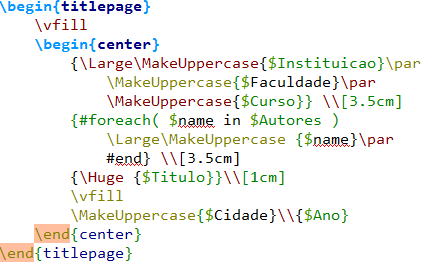
\includegraphics[width=3.07292in,height=1.96875in]{Cap02-img/Cap02-img001.png} 
\fonte{Autoria pr\'opria}} 
\end{figure}

{



\bigskip

\subsection[Writer2Latex]{ Writer2Latex}

\bigskip

{
\textrm{A API open source\ Writer2{\LaTeX} est\'a sendo utilizada no desenvolvimento do TCCTeX, pois reconhece todos
textos, tabelas e figuras que existem em um documento ODT (}\textrm{\textit{open document text}}\textrm{) e a partir
desse reconhecimento converte o arquivo para {\LaTeX}.}}

{
Essa convers\~ao s\'o \'e poss\'ivel\ por meio de um arquivo de configura\c{c}\~ao, onde dever\'a estar escrito como o
documento {\LaTeX} dever\'a se comportar, como por exemplo: n\~ao dever\'a existir par\'agrafos sem texto ou muitos
pulos de linha, cap\'itulos e sub cap\'itulos dever\~ao ser substitu\'idos pelo c\'odigo\ declarado, entre outras
coisas.}


\bigskip

{


\begin{figure}[H]
\caption{Exemplo de Configura\c{c}\~ao Writer2Latex}}
 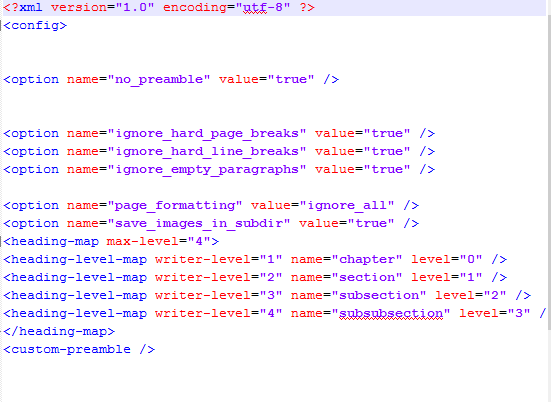
\includegraphics[width=4.8125in,height=3.51042in]{Cap02-img/Cap02-img002.png} 
\fonte{Autoria pr\'opria}} 
\end{figure}

{



\bigskip


\bigskip

{
\textrm{O Writer2Latex consegue fazer o seu papel de converter um arquivo\ }\textrm{\textit{Opendocument}}\textrm{\ para
{\LaTeX} muito bem, mas adiciona ao documento gerado v\'arias linhas de c\'odigo desnecess\'arias para nosso projeto,
al\'em disso n\~ao consegue reconhecer padr\~oes de legendas de figuras e tabelas, nem deixar o documento gerado no
padr\~ao ABNT, mas o TCCTeX conseguir\'a suprir todos estes problemas.}}